\documentclass[12pt,a4paper]{article}
\usepackage[pdftex]{graphicx}
\usepackage[spanish]{babel}
\usepackage[utf8]{inputenc}
\usepackage[T1]{fontenc}

\usepackage{amsmath}

\usepackage{listings}
\usepackage{xcolor}

\setlength{\parindent}{0pt} 

\lstset{
  language=R,
  basicstyle=\ttfamily\footnotesize,
  keywordstyle=\color{blue},
  commentstyle=\color{gray},
  stringstyle=\color{red},
  showstringspaces=false,
  breaklines=true
}

\hyphenation{op-tical net-works semi-conduc-tor}


\begin{document}

\title{Trabajo práctico 0: Procesamiento Digital de Imágenes}

\author{
    Diego Naranjo \\ Tecnológico de Costa Rica \\ l.naranjo.2@estudiantec.cr
    \and Gabriel Bonilla \\ Tecnológico de Costa Rica \\ g.bonilla.1@estudiantec.cr
    \and José Godínez \\ Tecnológico de Costa Rica \\ rodolfojose1996@estudiantec.cr
}


\markboth{Instituto Tecnológico de Costa Rica, Agosto~2025}%

\maketitle


\section{Sistemas lineales}

Demuestre si los siguientes sistemas $L\left\{ u(t)\right\} $ (con entrada $u(t)$ y salida $g(t)=L\left\{ u(t)\right\} $, y $h(t)$ una función cualquiera) son lineales o no lineales.

Para demostrar por contraejemplo programe la función que rechace la propiedad para 100 entradas generadas aleatoriamente:

\begin{itemize}
    \item $g\left(t\right)=\int_{-\infty}^{\infty}u(t)$
    \item $g\left(t\right)=\begin{cases} 1 & u(t)>0\\ 0 & u(t)\leq0 \end{cases}\,$
    \item $g\left(t\right)=\ln\left(u(t)\right)$
    \item $g\left(t\right)=\cos\left(u(t)\right)$
    \item $g\left(t\right)=\ln\left(5^{u(t)}\right)$
\end{itemize}

\subsection{$g(t)=\int^{\infty}_{-\infty}u(t)$}

\begin{itemize}
    \item  \textbf{Homogeneidad} ($L\{\alpha u(t)\} = \alpha L\{u(t)\}$):
    \begin{align*}
        L\{u(t)\} &= \int^{\infty}_{-\infty}u(t) \\
        L\{\alpha u(t)\} &= \int^{\infty}_{-\infty}\alpha u(t) \\
        L\{\alpha u(t)\} &= \alpha \int^{\infty}_{-\infty} u(t)\\
        L\{\alpha u(t)\} &= \alpha L\{u(t)\}
    \end{align*}
    \begin{itemize}
        \item \textbf{Aditividad} ($L\{u_1(t)+u_2(t)\}=L\{u_1(t)\}+ L\{u_2(t)\}$)
        \begin{align*}
            L\{u(t)\} &= \int^{\infty}_{-\infty}u(t) \\
            L\{u_1(t)+u_2(t)\} &=  \int^{\infty}_{-\infty}u_1(t)+u_2(t)\\
            L\{u_1(t)+u_2(t)\} &=  \int^{\infty}_{-\infty}u_1(t)+ \int^{\infty}_{-\infty}u_2(t)\\
            L\{u_1(t)+u_2(t)\} &= L\{u_1(t)\} + L\{u_2(t)\}
         \end{align*}
    \end{itemize}
    \item \textbf{Conclusión:} $g(t)$ cumple las condiciones para ser un sistema lineal.
\end{itemize}

\subsection{$
\quad g(t) =
\begin{cases}
1 & u(t) > 0 \\
0 & u(t) \leq 0
\end{cases}
$}

\begin{itemize}
    \item \textbf{Homogeneidad} ($L\{\alpha u(t)\} = \alpha L\{u(t)\}$): Analizando los casos:
    \begin{itemize}
        \item caso $u(t) > 0$, $\alpha > 0$: 
        \begin{align*}
            L\{\alpha u(t)\} &=  1\\
            L\{\alpha u(t)\} &\neq \alpha L\{ u(t)\}
        \end{align*}
    \end{itemize}
    Y evaluando un contraejemplo con $u(t) = 1$ y $\alpha = 2$
    \begin{align*}
        L\{\alpha u(t)\} &\stackrel{?}{=} \alpha L\{ u(t)\}\\
        L\{2\} &\stackrel{?}{=} 2 L\{ 1\}\\
        1 &\neq 2
    \end{align*}
    Y se pueden ver con más detalle en la sección \ref{subsec:contraejemplos}
    \item \textbf{Aditividad} ($L\{u_1(t)+u_2(t)\}=L\{u_1(t)\}+ L\{u_2(t)\}$): Analizamos el caso donde $u_1(t),u_2(t) >0$
    \begin{align*}
        L\{u_1(t)+u_2(t)\} &\stackrel{?}{=} L\{u_1(t)\}+L\{u_2(t)\}\\
        1 \neq 1+1
    \end{align*}
    \item \textbf{Conclusión:} $g(t)$ no cumple con las condiciones para ser un sistema lineal.

\end{itemize}

\subsection{$g(t)=\ln(u(t))$}

\begin{itemize}
    \item \textbf{Homogeneidad} ($L\{\alpha u(t)\} = \alpha L\{u(t)\}$)
    \begin{align*}
        L\{u(t)\} &= \ln(u(t))\\
        L\{\alpha u(t)\} &= \ln(\alpha u(t))\\
        L\{\alpha u(t)\} &= \ln(\alpha) + \ln(u(t))\\
        L\{\alpha u(t)\} &\neq \alpha L\{u(t)\}
    \end{align*}
    Y evaluando un contraejemplo con $u(t) = 1$ y $\alpha = 2$
    \begin{align*}
        L\{\alpha u(t)\} &\stackrel{?}{=} \alpha L\{ u(t)\}\\
        \ln(2) &\stackrel{?}{=} 2 \ln(1)\\
        0.69 &\neq 0
    \end{align*}
    \item \textbf{Aditividad} ($L\{u_1(t)+u_2(t)\}=L\{u_1(t)\}+ L\{u_2(t)\}$): Directamente por contra ejemplo
    \begin{align*}
        L\{u_1(t)+u_2(t)\} &\stackrel{?}{=} L\{u_1(t)\}+ L\{u_2(t)\}\\
        \ln (1+1) &\stackrel{?}{=} \ln (1) + \ln (1) \\
        \ln (2) &\neq 0 \\
    \end{align*}
    \item \textbf{Conclusión:} $g(t)$ no cumple con las condiciones para ser un sistema lineal y se pueden ver con más detalle los contraejemplos en la sección \ref{subsec:contraejemplos}
\end{itemize}

\subsection{$g(t)=\cos(u(t))$}

\begin{itemize}
    \item \textbf{Homogeneidad} ($L\{\alpha u(t)\} = \alpha L\{u(t)\}$): Directamente por contraejemplo:
        \begin{align*}
            L\{\alpha u(t)\} &\stackrel{?}{=} \ln(\alpha u(t))\\
            \cos (2\pi) &\stackrel{?}{=} 2 \cos (\pi)
            1 \neq -2 
        \end{align*}
    \item \textbf{Aditividad} ($L\{u_1(t)+u_2(t)\}=L\{u_1(t)\}+ L\{u_2(t)\}$)
    \begin{align*}
        L\{u(t)\} &= \cos(u(t))\\
        L\{u_1(t)+u_2(t)\} &= \cos (u_1(t)+u_2(t))\\
        \cos(a+b) &= \cos(a)\cos(b)-\sin(a)\sin(b)\\
        L\{u_1(t)+u_2(t)\} &= \cos(u_1(t))\cos(u_2(t))-\sin(u_1(t))\sin(u_2(t))\\
        L\{u_1(t)+u_2(t)\} &\neq L\{u_1(t)\}+L\{u_2(t)\} 
    \end{align*}
    Y verificando lo obtenido con un contrajemplo:
    \begin{align*}
        L\{u_1(t)+u_2(t)\} &\stackrel{?}{=} L\{u_1(t)\}+ L\{u_2(t)\}\\
        \cos(1+2) &\stackrel{?}{=} \cos(1) + \cos(2)\\
         -0.99 &\neq 0.54 + -0.41
    \end{align*}
    \item \textbf{Conclusión:} $g(t)$ no cumple con las condiciones para ser un sistema lineal y se pueden ver con más detalle los contraejemplos en la sección \ref{subsec:contraejemplos}
\end{itemize}

\subsection{$g(t)=\ln(5^{u(t)})$}

\begin{itemize}
    \item \textbf{Homogeneidad} ($L\{\alpha u(t)\} = \alpha L\{u(t)\}$)
    \begin{align*}
        g(t)&=\ln(5^{u(t)})\\
        g(t) &= u(t)\ln(5), \text{con} \ln(a^b)=b\ln(a)\\
        L\{u(t)\} &= u(t)\ln(5)\\
        L\{\alpha u(t)\} &= \alpha u(t) \ln(5)\\
        L\{\alpha u(t)\} &= \alpha L\{u(t)\}
    \end{align*}
    \item \textbf{Aditividad} ($L\{u_1(t)+u_2(t)\}=L\{u_1(t)\}+ L\{u_2(t)\}$)
        \begin{align*}
        L\{u(t)\} &= u(t)\ln(5)\\
        L\{u_1(t)+u_2(t)\} &= (u_1(t)+u_2(t)) \ln(5)\\
        L\{u_1(t)+u_2(t)\} &= \ln(5)u_1(t)+\ln(5)u_2(t)\\
        L\{u_1(t)+u_2(t)\} &= L\{u_1(t)\}+L\{u_2(t)\}
    \end{align*}
    \item \textbf{Conclusión}: $g(t)$ sí cumple con los criterios para ser un sistema lineal.
\end{itemize}

\subsection{Verificaciones de contraejemplos}
\label{subsec:contraejemplos}

Para cada uno de los sistemas que se determinaron como no lineales (b, c y d), se realizó:
\begin{itemize}
    \item Generación de conjuntos $u_1$, $u_2$ con tamaño 100 cada uno y un escalar $\alpha$. Para la función del $\ln$, se acotaron los valores menores a 0 como $0.00001$ por terminos de indefinición.
    \item Vectorialmente con torch se revisó la aditividad $L\{u_1(t)+u_2(t)\} &\stackrel{?}{=} L\{u_1(t)\}+ L\{u_2(t)\}$
    \item Vectorialmente se revisó la homogeneidad $L\{\alpha u(t)\} = \alpha L\{u(t)\}$
\end{itemize}

Los resultados obtenidos en la figura \ref{fig:counterexamples}

\begin{figure*}[h!]
    \centering
    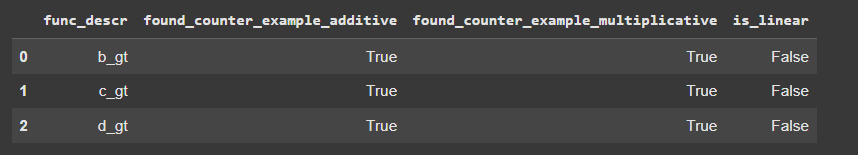
\includegraphics[width=\textwidth]{../img/counterexamples.PNG}
    \caption{Resultados de la prueba automatizada de búsqueda de contraejemplos en el análisis de los posibles sistemas lineales, donde los sistemas b, c y d se les encontró que no cumplen lo necesario para ser considerados lineales.}
    \label{fig:counterexamples}
\end{figure*}

\section{Interpolación bilineal}

\subsection{Proceso matemático}

Para interpolar bilinealmente el valor de la coordenada $z$ para cada uno de los puntos de una submatriz, se requiere identificar un plano que pasa por 3 puntos ya conocidos, en este caso de las esquinas. Para ello, tenemos que recordar que un plano está definido por la ecuación $ax + by + cz + d = 0$, siendo $a$, $b$ y $c$ los coeficientes del plano, $d$ su offset y $x$, $y$ y $z$ las coordenadas de un punto en $R^3$. \\

Dicho esto, para calcular la ecuación del plano en cada una de las submatrices, vamos tomar 3 de sus puntos conocidos. Los vamos a denominar $P_1$, $P_2$ y $P_3$. Con ellos, vamos a calcular 2 vectores directores plano:

\[
\vec{(P_1 - P_2)} = [x_1 - x_2, y_1 - y_2, z_1 - z_2]
\]
\[
\vec{(P_2 - P_3)} = [x_2 - x_3, y_2 - y_3, z_2 - z_3]
\]

Al estos vectores estar en el plano, sirven para obtener un vector normal del mismo, y así mismo, sus coeficientes. Esto se hace mediante el producto cruz de los vectores:

\[
\vec{(P_1 - P_2)} \times \vec{(P_2 - P_3)} = \vec{n}
\]

Una vez obtenido el vector normal $\vec{n}$, podemos definir la exuación del plano de la siguiente manera:

\[
n_1x + n_2y + n_3z + d = 0
\]

Para determinar el valor de $d$, simplemente se sustituyen, en la ecuación, los valores de $x$, $y$ y $z$ por las coordenadas de un punto conocido del plano y se despeja $d$. En este caso, el punto escogido puede ser cualquiera de $P_1$, $P_2$ y $P_3$:

\[
d = -(n_1P_{1_x} + n_2P_{1_y} + n_3P_{1_z})
\]

Ya se tienen todos los valores necesarios para poder despejar y encontrar la coordenada $z$ de un punto utilizando la ecuación del plano, en casos que se conozcan sus coordenadas $x$, $y$: 

\[
z = \frac{(-d - n_1x - n_2y)}{n_3}
\]

\subsection{Ejemplo}

La siguiente matriz $U$ representa una submatriz de una imagen a la que se le aplicó un aumento con $\alpha = 2$:

\[
U =
    \begin{bmatrix}
    1 & ? & 2 \\
    ? & ? & ? \\
    3 & ? & 4
    \end{bmatrix}
\]

Dada la submatriz $U$, se tienen los puntos conocidos:

\[
P_1 = [0,0,1], P_2 [2,0,3], P_3 = [2,2,4]
\]

Se definen los 2 vectores directores como:

\[
\vec{P_1 - P_2} = [-2,0-2], \vec{P_2 - P_3} = [2,2,4]
\]

Se calcula el vector normal:

\[
\vec{P_1 - P_2} \times \vec{P_2 - P_3} = [-4,-2,4]
\]

Se utiliza $P_1$ para obtener el valor de $d$:

\[
d = -((-4 \cdot 0) + (-2\cdot 0) + (4\cdot 1)) = -4
\]

Por último, se calcula la coordenada $z$ para cada uno de los valores faltantes de la submatriz:

\begin{align*}
\textit{Para } (0,1,z), \; & z = \frac{(4 + (4 \cdot 0) + (2 \cdot 1))}{4} = 1.5 \\[6pt]
\textit{Para } (1,0,z), \; & z = \frac{(4 + (4 \cdot 1) + (2 \cdot 0))}{4} = 2 \\[6pt]
\textit{Para } (1,1,z), \; & z = \frac{(4 + (4 \cdot 1) + (2 \cdot 1))}{4} = 2.5 \\[6pt]
\textit{Para } (1,2,z), \; & z = \frac{(4 + (4 \cdot 1) + (2 \cdot 2))}{4} = 3 \\[6pt]
\textit{Para } (2,1,z), \; & z = \frac{(4 + (4 \cdot 2) + (2 \cdot 1))}{4} = 3.5
\end{align*}

La submatriz $U$ quedaría de la siguiente manera:

\[
U =
    \begin{bmatrix}
    1 & 1.5 & 2 \\
    2 & 2.5 & 3 \\
    3 & 3.5 & 4
    \end{bmatrix}
\]


\end{document}


